\section{Heurística de Búsqueda Local}

\subsection{Algoritmo}

%\indent El algoritmo de búsqueda local que implementamos parte de una solución obtenida mediante el algoritmo constructivo goloso mostrado anteriormente. A partir de allí recorre cada nodo y chequea si cambiándole el color por el de alguno de sus vecinos si aumenta el impacto en H (siempre y cuando se esté en el contexto de un coloreo válido en G). De esta manera, comienza a generar un nuevo coloreo que parte de aquél obtenido por el algoritmo goloso. Luego de terminar de generarlo lo devuelve. \\

\indent El algoritmo de búsqueda local que implementamos parte de una solución obtenidad por el algoritmo contructivo goloso aleatorio que desarrollamos y detallamos en la sección anterior de este Trabajo Práctico. Se recibe un parámetro que será el valor $porcentaje$, utilizado a la hora de aplicar el algoritmo goloso como solución inicial.\\
\indent Una vez obtenida esta solución base, se procede a iterar explorando el espacio de las soluciones vecinas.\\
\indent Para ello, fue menester definir la vecindad entre soluciones. Definimos la vecindad de una solución en el contexto del algoritmo de búsqueda local como aquellos coloreos válidos de G que se obtienen de modificar el color de algún nodo de dicha solución por el color de alguno de los vecinos de ese nodo en el grafo H. Resultó natural definir la vecindad de esta manera pensando en el significado de Impacto de un coloreo de G en H, dado que lo que buscamos es que para un coloreo válido de G la mayor cantidad de nodos vecinos entre sí en H estén coloreados del mismo color.\\

\indent Una vez hechos estos comentarios, nos abocamos a describir el funcionamiento de nuestra implementación del algoritmo de búsqueda local para resolver el problema del coloreo de máximo impacto de G en H.\\
\indent Como mencionamos anteriormente, partimos de una solución obtenida mediante nuestra implementación del algoritmo constructivo goloso, ejecutado con el parámetro $porcentaje$ que está búsqueda local recibe por parámetro. Una vez obtenida esa solución, se comienza a recorrer sus vecinas.\\
\indent Para ello, se comienza a iterar en los nodos de H. Por cada nodo, se recorren sus vecinos en H y se analiza si se mejora el impacto cambiándole el color a ese nodo por el de alguno de sus vecinos (siempre y cuando dicho coloreo sea válido en G). En caso de que se obtuviese un mejor impacto, se actualiza la solución con el cambio propuesto y se continúa iterando en los vecinos de ese nodo, esta vez comparando la solución parcial con la nueva solución obtenida. Una vez recorridos todos los vecinos de ese nodo en H, se pasa a otro nodo y se repite el proceso, actualizando la solución en caso de ser necesario con los criterios mencionados.\\
\indent El resultado es entonces una solución que se obtuvo de ir modificando la primera solución obtenida con el algoritmo goloso. Por la manera en que fuimos operando, podemos estar seguros de que si la solución final es diferente a la solución inicial de la que se partió, entonces el impacto del tal coloreo de G en H es mayor al de la solución golosa. En el caso en que ninguna de las soluciones vecinas de la solución golosa mejore el impacto se devuelve entonces la solución inicial.\\
\indent Hay que tener en cuenta que al ser una búsqueda local, se termina \textit{cayendo} en un mínimo local, con lo que probablemente no se obtenga la solución óptima del problema.


\begin{algorithm}[H]
\caption{} 
\begin{codebox}
\Procname{$\proc{maximoImpactoLocal}(Grafo$ g$, Grafo$ h$, double $ porcentaje$)$}

\li
\li vector$<$unsigned int$>$ impactoGoloso  $\gets$ maximoImpactoGoloso(g,h,porcentaje)
\li unsigned int impactoParcial $\gets$ impactoGoloso[0];
\li vector$<$unsigned int$>$ coloreo(n);
\li
\li vector$<$unsigned int$>$ solucionFinal(n+1);
\li
\li \For i desde 1 hasta n \Do
    
\li 	coloreo[i] $\gets$ impactoGoloso[i]
    
    \End
\li

\li unsigned int nuevoImpacto $\gets$ 0
\li
\li	\For i desde 1 hasta n \Do
	
\li
\li		vector$<$unsigned int$>$ vecinos $\gets$ vecinos del nodo i en h
\li
\li 	\For j desde 1 hasta la cantidad de vecinos de i en h \Do

\li				unsigned int color = coloreo[vecinos[j]]
\li
\li				\If pintar al nodo i de $color$ es legal \Do			
\li						vector$<$unsigned int$>$ nuevoColoreo $\gets$ \quad $coloreo$
\li						nuevoColoreo[i]$ \gets$ \quad $color$
\li                		nuevoImpacto $ \gets$ \quad $h.impacto(nuevoColoreo)$
\li
\li                		\If nuevoImpacto $>$ impactoParcial \Do
                
\li                			coloreo[i] $\gets$ \quad $color$
\li                   			impactoParcial $\gets$ \quad $nuevoImpacto$
                   		\End
\li
                \End
        \End
    \End

\li
%\li		impactoGoloso[0] $\gets$ \quad $impactoParcial$
\li 		solucionFinal[0] $\gets$ \quad $impactoParcial$
\li
\li \For i desde 0 hasta n \Do
%\li		impactoGoloso[i+1]=coloreo[i]
\li		solucionFinal[i+1]=coloreo[i]
	\End    

\li
%\li return impactoGoloso
\li return solucionFinal
\End
\end{codebox}
\end{algorithm}

\subsection{Análisis de complejidad}

\indent Veamos la complejidad de maximoImpactoLocal. Primero se calcula una solución con maximoImpactoGoloso. Como mencionamos en el apartado correspondiente eso cuesta O(n*(n+m)+ $n^{3}$). \\
\indent Luego, se copia el coloreo que se obtuvo de maximoImpactoGoloso en O(n).\\
\indent A continuación se itera sobre la cantidad de nodos de H. En cada iteración se copian los vecinos del nodo en el que estamos ahora. Como dicho nodo puede tener a lo sumo n-1 vecinos, eso cuesta O(n). Luego,se itera sobre los vecinos del nodo y por cada vecino del nodo se decide en O(n+m) si se va a pintar el nodo del mismo color que su vecino. Dicha decisión se fundamenta en si cambiar el color genera un coloreo válido en G y si aumenta el impacto H. Entonces,el costo del ciclo interior cuesta O(n*(n+m)). Por lo tanto, el ciclo que lo engloba cuesta O($n^{2}$*(n+m)).\\
\indent Luego de terminar de iterar se guarda el coloreo parcial con un costo de O(n).\\
\indent Entonces, maximoImpactoLocal cuesta O(n*(n+m)+ $n^{3}$ +$ n^{2}$*(n+m)).\\

\subsection{Experimentación y Resultados}

\quad A continuación analizaremos el costo temporal de la búsqueda local. Al igual que antes, testeamos con grafos generados al azar, con grafos estrellas no uniformes y grafos web de 4 vértices.

\quad Se midieron los tiempos en corridas de  5 a 100 nodos con 50 repeticiones para cada cantidad de nodos y se las comparó con la cota teórica calculada anteriormente.


\begin{figure}[H]
	\centering
	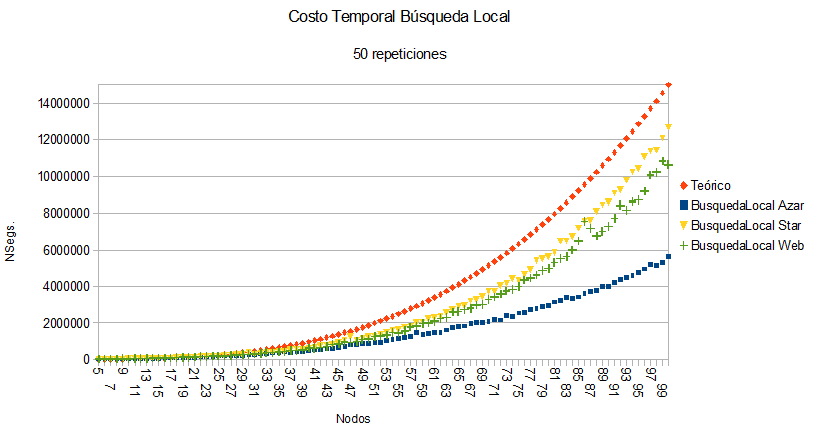
\includegraphics[scale=0.6]{timingBLocal.png}
\caption{Costos}
\end{figure}

\quad

\quad Se observa que se cumple con la cota del peor caso calculada.

\quad A diferencia de la heurística golosa, se puede ver que con los tres tipos de grafos se obtuvieron diferentes resultados.

\quad Con la que menor costos temporales se obtuvo fue con los grafos generados al azar. En cambio, vemos que con los grafos estrella el costo aumenta considerablemente. En menor medida ocurre con los grafos de red de 4 nodos. 

\quad Esto se debe a que estos dos últimos tipos de grafos en general son menos \textit{densos} que los grafos generados aleatoriamente. Como nuestra heurística de búsqueda local busca cambiar el color de un nodo por otro color legal (de algún vecino en el grafo H) en estos grafos menos densos hay mayor opciones por lo que se itera y prueba más veces.

\quad Si bien las cotas teóricas de las heurísticas golosa y de búsqueda local son las mismas, las constante que las multiplica son distintas, siendo mayor la de esta última ya que requiere más cálculo computacional que proviene de explorar la vecindad de la solución golosa usada como base.